\section*{Metodi con rappresentazione grafica}
I prossimi metodi che verranno descritti utilizzeranno lo strumento Octave
per la rappresentazione grafica dei metodi per illustrare in modo pi\`u chiaro
il comportamento del metodo iterativo in questione.

Tutti i grafici hanno uno schema comune, ovvero sono composti da tre curve:
\begin{itemize}
  \item la curva cyan rappresenta la funzione $f(x)$ che si sta studiando
  \item la curva blu, composta da pochi simboli '$+$', rappresenta punti
  calcolati dal metodo per convergere allo zero $x^{*}$
  \item la curva rossa rappresenta il comportamento del metodo, visualizzando
  la sequenza con cui si procede per convergere alla soluzione
\end{itemize}

\section{Metodo di bisezione}
\label{sec:metodoDiBisezione}
Riporto il codice di pagina 23:
\begin{lstlisting}
octave:12> p = poly([1.1*ones(1,20) pi])
p =
 Columns 1 through 6:
   1.0000e+00  -2.5142e+01   2.9902e+02  -2.2396e+03   1.1860e+04  -4.7254e+04
 Columns 7 through 12:
   1.4711e+05  -3.6678e+05   7.4461e+05  -1.2444e+06   1.7234e+06  -1.9847e+06
 Columns 13 through 18:
   1.9008e+06  -1.5096e+06   9.8794e+05  -5.2718e+05   2.2572e+05  -7.5702e+04
 Columns 19 through 22:
   1.9159e+04  -3.4410e+03   3.9100e+02  -2.1135e+01
octave:13> polyval(p,pi)
ans =  2.0207e-04
\end{lstlisting}
Lo scopo della funzione $poly(r)$ \`e quello di creare un vettore di coefficienti
di un polinomio $p$, tale che le radici di $p$ appartengono al vettore $r$ 
($poly: Root[] \rightarrow PolynomialCoefficient[]$).
Valutando quindi il polinomio in una sua radice (\emph{octave:13}) in aritmetica
esatta dovrei ottenere 0, mentre in aritmetica finita non \`e vero 
($p(\pi) = ans =  2.0207e-04 \not = 0$).

\begin{exercise}
Implementare il metodo di bisezione ed applicarlo alla funzione $\sin(x)$ 
con intervallo iniziale $[2, 5]$ ed una tollerenza $tol_{X} = 10^{-14}$.
\end{exercise}
Per l'implementazione del codice vedere \nameref{sec:bisectionIterativeMethod}.
\begin{lstlisting}
octave:45> [x, i, imax, ascisse] = bisectionMethod('sin', 2, 5, e^-14)
x =  3.14159250259399e+00
i =  2.10000000000000e+01
imax =  2.20000000000000e+01
ascisse =
 Columns 1 through 3:
   3.50000000000000e+00   2.75000000000000e+00   3.12500000000000e+00
 Columns 4 through 6:
   3.31250000000000e+00   3.21875000000000e+00   3.17187500000000e+00
 Columns 7 through 9:
   3.14843750000000e+00   3.13671875000000e+00   3.14257812500000e+00
 Columns 10 through 12:
   3.13964843750000e+00   3.14111328125000e+00   3.14184570312500e+00
 Columns 13 through 15:
   3.14147949218750e+00   3.14166259765625e+00   3.14157104492188e+00
 Columns 16 through 18:
   3.14161682128906e+00   3.14159393310547e+00   3.14158248901367e+00
 Columns 19 through 21:
   3.14158821105957e+00   3.14159107208252e+00   3.14159250259399e+00
octave:46> xsin = min(ascisse):0.01:max(ascisse)
octave:47> ysin = feval('sin', xsin)
octave:48> [prepX, prepY] = prepareForPlottingMethodSegments(ascisse, "sin", "")
octave:49> plot(xsin, ysin, "c", ascisse, feval('sin', ascisse), "b+", prepX, prepY, "r")
octave:50> print 'bisectionPlotOutput.tex' '-dTex' '-S800, 600'
\end{lstlisting}
Si raggiunge la tolleranza richiesta in 21 passi, uno in meno delle iterazioni
massime possibili. Questo l'output del comando \emph{octave:50}:
\begin{center}
% GNUPLOT: LaTeX picture with Postscript
\begingroup
  \makeatletter
  \providecommand\color[2][]{%
    \GenericError{(gnuplot) \space\space\space\@spaces}{%
      Package color not loaded in conjunction with
      terminal option `colourtext'%
    }{See the gnuplot documentation for explanation.%
    }{Either use 'blacktext' in gnuplot or load the package
      color.sty in LaTeX.}%
    \renewcommand\color[2][]{}%
  }%
  \providecommand\includegraphics[2][]{%
    \GenericError{(gnuplot) \space\space\space\@spaces}{%
      Package graphicx or graphics not loaded%
    }{See the gnuplot documentation for explanation.%
    }{The gnuplot epslatex terminal needs graphicx.sty or graphics.sty.}%
    \renewcommand\includegraphics[2][]{}%
  }%
  \providecommand\rotatebox[2]{#2}%
  \@ifundefined{ifGPcolor}{%
    \newif\ifGPcolor
    \GPcolortrue
  }{}%
  \@ifundefined{ifGPblacktext}{%
    \newif\ifGPblacktext
    \GPblacktexttrue
  }{}%
  % define a \g@addto@macro without @ in the name:
  \let\gplgaddtomacro\g@addto@macro
  % define empty templates for all commands taking text:
  \gdef\gplbacktext{}%
  \gdef\gplfronttext{}%
  \makeatother
  \ifGPblacktext
    % no textcolor at all
    \def\colorrgb#1{}%
    \def\colorgray#1{}%
  \else
    % gray or color?
    \ifGPcolor
      \def\colorrgb#1{\color[rgb]{#1}}%
      \def\colorgray#1{\color[gray]{#1}}%
      \expandafter\def\csname LTw\endcsname{\color{white}}%
      \expandafter\def\csname LTb\endcsname{\color{black}}%
      \expandafter\def\csname LTa\endcsname{\color{black}}%
      \expandafter\def\csname LT0\endcsname{\color[rgb]{1,0,0}}%
      \expandafter\def\csname LT1\endcsname{\color[rgb]{0,1,0}}%
      \expandafter\def\csname LT2\endcsname{\color[rgb]{0,0,1}}%
      \expandafter\def\csname LT3\endcsname{\color[rgb]{1,0,1}}%
      \expandafter\def\csname LT4\endcsname{\color[rgb]{0,1,1}}%
      \expandafter\def\csname LT5\endcsname{\color[rgb]{1,1,0}}%
      \expandafter\def\csname LT6\endcsname{\color[rgb]{0,0,0}}%
      \expandafter\def\csname LT7\endcsname{\color[rgb]{1,0.3,0}}%
      \expandafter\def\csname LT8\endcsname{\color[rgb]{0.5,0.5,0.5}}%
    \else
      % gray
      \def\colorrgb#1{\color{black}}%
      \def\colorgray#1{\color[gray]{#1}}%
      \expandafter\def\csname LTw\endcsname{\color{white}}%
      \expandafter\def\csname LTb\endcsname{\color{black}}%
      \expandafter\def\csname LTa\endcsname{\color{black}}%
      \expandafter\def\csname LT0\endcsname{\color{black}}%
      \expandafter\def\csname LT1\endcsname{\color{black}}%
      \expandafter\def\csname LT2\endcsname{\color{black}}%
      \expandafter\def\csname LT3\endcsname{\color{black}}%
      \expandafter\def\csname LT4\endcsname{\color{black}}%
      \expandafter\def\csname LT5\endcsname{\color{black}}%
      \expandafter\def\csname LT6\endcsname{\color{black}}%
      \expandafter\def\csname LT7\endcsname{\color{black}}%
      \expandafter\def\csname LT8\endcsname{\color{black}}%
    \fi
  \fi
  \setlength{\unitlength}{0.0500bp}%
  \begin{picture}(7680.00,5760.00)%
    \gplgaddtomacro\gplbacktext{%
      \colorrgb{0.00,0.00,0.00}%
      \put(866,634){\makebox(0,0)[r]{\strut{}-0.4}}%
      \colorrgb{0.00,0.00,0.00}%
      \put(866,1221){\makebox(0,0)[r]{\strut{}-0.3}}%
      \colorrgb{0.00,0.00,0.00}%
      \put(866,1807){\makebox(0,0)[r]{\strut{}-0.2}}%
      \colorrgb{0.00,0.00,0.00}%
      \put(866,2394){\makebox(0,0)[r]{\strut{}-0.1}}%
      \colorrgb{0.00,0.00,0.00}%
      \put(866,2981){\makebox(0,0)[r]{\strut{}0}}%
      \colorrgb{0.00,0.00,0.00}%
      \put(866,3567){\makebox(0,0)[r]{\strut{}0.1}}%
      \colorrgb{0.00,0.00,0.00}%
      \put(866,4154){\makebox(0,0)[r]{\strut{}0.2}}%
      \colorrgb{0.00,0.00,0.00}%
      \put(866,4740){\makebox(0,0)[r]{\strut{}0.3}}%
      \colorrgb{0.00,0.00,0.00}%
      \put(866,5327){\makebox(0,0)[r]{\strut{}0.4}}%
      \colorrgb{0.00,0.00,0.00}%
      \put(998,414){\makebox(0,0){\strut{}2.6}}%
      \colorrgb{0.00,0.00,0.00}%
      \put(2188,414){\makebox(0,0){\strut{}2.8}}%
      \colorrgb{0.00,0.00,0.00}%
      \put(3379,414){\makebox(0,0){\strut{}3}}%
      \colorrgb{0.00,0.00,0.00}%
      \put(4569,414){\makebox(0,0){\strut{}3.2}}%
      \colorrgb{0.00,0.00,0.00}%
      \put(5760,414){\makebox(0,0){\strut{}3.4}}%
      \colorrgb{0.00,0.00,0.00}%
      \put(6950,414){\makebox(0,0){\strut{}3.6}}%
    }%
    \gplgaddtomacro\gplfronttext{%
    }%
    \gplbacktext
    \put(0,0){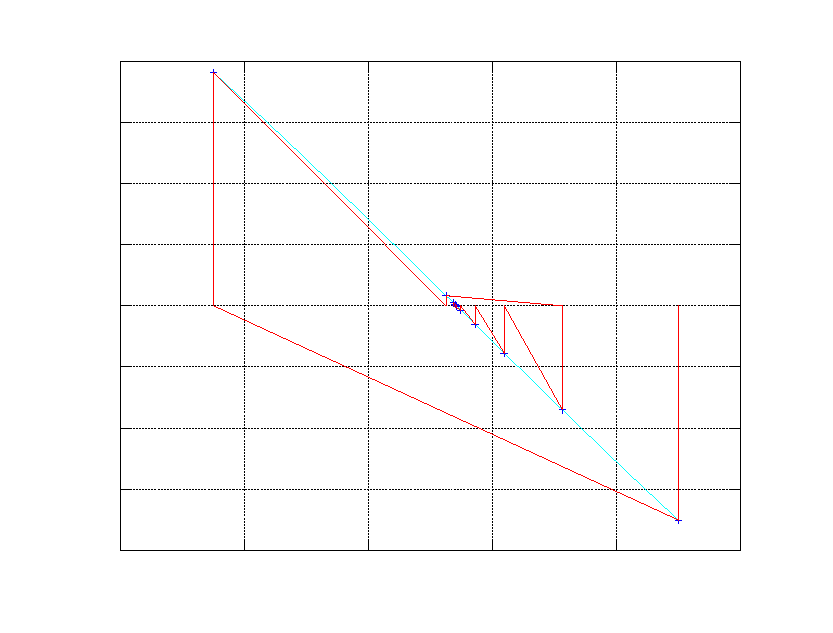
\includegraphics{RadiciEquazione/bisectionPlotOutput}}%
    \gplfronttext
  \end{picture}%
\endgroup

\end{center}

\begin{exercise}
Implementare il metodo di bisezione ed applicarlo alla funzione $\sin(x)$ 
con intervallo iniziale $[-0.1, 7]$, in modo da avere due zeri nell'
intervallo di confidenza, ed una tollerenza $tol_{X} = 10^{-14}$.
\end{exercise}
Per l'implementazione del codice vedere \nameref{sec:bisectionIterativeMethod}.
\begin{lstlisting}
octave:51> [x, i, imax, ascisse] = bisectionMethod('sin', -0.1, 7, e^-14)
x =  6.28318557739258e+00
i =  1.70000000000000e+01
imax =  2.40000000000000e+01
ascisse =
 Columns 1 through 3:
   3.45000000000000e+00   5.22500000000000e+00   6.11250000000000e+00
 Columns 4 through 6:
   6.55625000000000e+00   6.33437500000000e+00   6.22343750000000e+00
 Columns 7 through 9:
   6.27890625000000e+00   6.30664062500000e+00   6.29277343750000e+00
 Columns 10 through 12:
   6.28583984375000e+00   6.28237304687500e+00   6.28410644531250e+00
 Columns 13 through 15:
   6.28323974609375e+00   6.28280639648438e+00   6.28302307128906e+00
 Columns 16 and 17:
   6.28313140869141e+00   6.28318557739258e+00
octave:52> xsin = min(ascisse):0.01:max(ascisse)
octave:53> ysin = feval('sin', xsin)
octave:54> [prepX, prepY] = prepareForPlottingMethodSegments(ascisse, "sin", "")
octave:55> plot(xsin, ysin, "c", ascisse, feval('sin', ascisse), "b+", prepX,
prepY, "r") 
octave:56> print 'bisectionWithTwoRootsPlotOutput.tex' '-dTex' '-S800, 600'
\end{lstlisting}
Si raggiunge la tolleranza richiesta in 17 passi, sette in meno delle iterazioni massime possibili. 
Questo l'output del comando \emph{octave:56}:
\begin{center}
% GNUPLOT: LaTeX picture with Postscript
\begingroup
  \makeatletter
  \providecommand\color[2][]{%
    \GenericError{(gnuplot) \space\space\space\@spaces}{%
      Package color not loaded in conjunction with
      terminal option `colourtext'%
    }{See the gnuplot documentation for explanation.%
    }{Either use 'blacktext' in gnuplot or load the package
      color.sty in LaTeX.}%
    \renewcommand\color[2][]{}%
  }%
  \providecommand\includegraphics[2][]{%
    \GenericError{(gnuplot) \space\space\space\@spaces}{%
      Package graphicx or graphics not loaded%
    }{See the gnuplot documentation for explanation.%
    }{The gnuplot epslatex terminal needs graphicx.sty or graphics.sty.}%
    \renewcommand\includegraphics[2][]{}%
  }%
  \providecommand\rotatebox[2]{#2}%
  \@ifundefined{ifGPcolor}{%
    \newif\ifGPcolor
    \GPcolortrue
  }{}%
  \@ifundefined{ifGPblacktext}{%
    \newif\ifGPblacktext
    \GPblacktexttrue
  }{}%
  % define a \g@addto@macro without @ in the name:
  \let\gplgaddtomacro\g@addto@macro
  % define empty templates for all commands taking text:
  \gdef\gplbacktext{}%
  \gdef\gplfronttext{}%
  \makeatother
  \ifGPblacktext
    % no textcolor at all
    \def\colorrgb#1{}%
    \def\colorgray#1{}%
  \else
    % gray or color?
    \ifGPcolor
      \def\colorrgb#1{\color[rgb]{#1}}%
      \def\colorgray#1{\color[gray]{#1}}%
      \expandafter\def\csname LTw\endcsname{\color{white}}%
      \expandafter\def\csname LTb\endcsname{\color{black}}%
      \expandafter\def\csname LTa\endcsname{\color{black}}%
      \expandafter\def\csname LT0\endcsname{\color[rgb]{1,0,0}}%
      \expandafter\def\csname LT1\endcsname{\color[rgb]{0,1,0}}%
      \expandafter\def\csname LT2\endcsname{\color[rgb]{0,0,1}}%
      \expandafter\def\csname LT3\endcsname{\color[rgb]{1,0,1}}%
      \expandafter\def\csname LT4\endcsname{\color[rgb]{0,1,1}}%
      \expandafter\def\csname LT5\endcsname{\color[rgb]{1,1,0}}%
      \expandafter\def\csname LT6\endcsname{\color[rgb]{0,0,0}}%
      \expandafter\def\csname LT7\endcsname{\color[rgb]{1,0.3,0}}%
      \expandafter\def\csname LT8\endcsname{\color[rgb]{0.5,0.5,0.5}}%
    \else
      % gray
      \def\colorrgb#1{\color{black}}%
      \def\colorgray#1{\color[gray]{#1}}%
      \expandafter\def\csname LTw\endcsname{\color{white}}%
      \expandafter\def\csname LTb\endcsname{\color{black}}%
      \expandafter\def\csname LTa\endcsname{\color{black}}%
      \expandafter\def\csname LT0\endcsname{\color{black}}%
      \expandafter\def\csname LT1\endcsname{\color{black}}%
      \expandafter\def\csname LT2\endcsname{\color{black}}%
      \expandafter\def\csname LT3\endcsname{\color{black}}%
      \expandafter\def\csname LT4\endcsname{\color{black}}%
      \expandafter\def\csname LT5\endcsname{\color{black}}%
      \expandafter\def\csname LT6\endcsname{\color{black}}%
      \expandafter\def\csname LT7\endcsname{\color{black}}%
      \expandafter\def\csname LT8\endcsname{\color{black}}%
    \fi
  \fi
  \setlength{\unitlength}{0.0500bp}%
  \begin{picture}(7680.00,5760.00)%
    \gplgaddtomacro\gplbacktext{%
      \colorrgb{0.00,0.00,0.00}%
      \put(866,634){\makebox(0,0)[r]{\strut{}-1}}%
      \colorrgb{0.00,0.00,0.00}%
      \put(866,1304){\makebox(0,0)[r]{\strut{}-0.8}}%
      \colorrgb{0.00,0.00,0.00}%
      \put(866,1975){\makebox(0,0)[r]{\strut{}-0.6}}%
      \colorrgb{0.00,0.00,0.00}%
      \put(866,2645){\makebox(0,0)[r]{\strut{}-0.4}}%
      \colorrgb{0.00,0.00,0.00}%
      \put(866,3316){\makebox(0,0)[r]{\strut{}-0.2}}%
      \colorrgb{0.00,0.00,0.00}%
      \put(866,3986){\makebox(0,0)[r]{\strut{}0}}%
      \colorrgb{0.00,0.00,0.00}%
      \put(866,4657){\makebox(0,0)[r]{\strut{}0.2}}%
      \colorrgb{0.00,0.00,0.00}%
      \put(866,5327){\makebox(0,0)[r]{\strut{}0.4}}%
      \colorrgb{0.00,0.00,0.00}%
      \put(998,414){\makebox(0,0){\strut{}3}}%
      \colorrgb{0.00,0.00,0.00}%
      \put(1742,414){\makebox(0,0){\strut{}3.5}}%
      \colorrgb{0.00,0.00,0.00}%
      \put(2486,414){\makebox(0,0){\strut{}4}}%
      \colorrgb{0.00,0.00,0.00}%
      \put(3230,414){\makebox(0,0){\strut{}4.5}}%
      \colorrgb{0.00,0.00,0.00}%
      \put(3974,414){\makebox(0,0){\strut{}5}}%
      \colorrgb{0.00,0.00,0.00}%
      \put(4718,414){\makebox(0,0){\strut{}5.5}}%
      \colorrgb{0.00,0.00,0.00}%
      \put(5462,414){\makebox(0,0){\strut{}6}}%
      \colorrgb{0.00,0.00,0.00}%
      \put(6206,414){\makebox(0,0){\strut{}6.5}}%
      \colorrgb{0.00,0.00,0.00}%
      \put(6950,414){\makebox(0,0){\strut{}7}}%
    }%
    \gplgaddtomacro\gplfronttext{%
    }%
    \gplbacktext
    \put(0,0){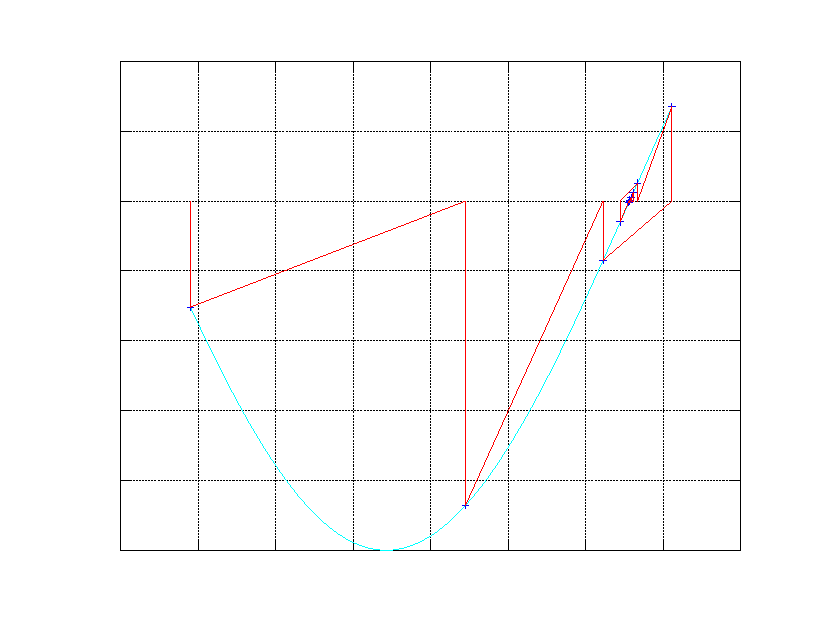
\includegraphics{RadiciEquazione/bisectionWithTwoRootsPlotOutput}}%
    \gplfronttext
  \end{picture}%
\endgroup

\end{center}

Da questo esercizio si vede che il metodo di bisezione converge comunque
ad una radice (in questa applicazione a $2\pi$), anche nel caso in cui
nell'intervallo di confidenza ci sono pi\`u zeri della funzione.





\section{Metodo di Newton}
\label{sec:metodoDiNewton}

\begin{exercise}
Implementare il metodo di newton ed applicarlo alla funzione \emph{singleZero},
con innesco iniziale $x_{0} = 7$, una tollerenza assoluta e relativa
$tol_{X} = rTol_{X} = 10^{-14}$ ed un numero massimo di iterazioni
$i_{max} = 10^{2}$.
\end{exercise}
Per l'implementazione del codice vedere \nameref{sec:newtonIterativeMethod}.
\begin{lstlisting}
octave:112> [x, i, ascisse] = newtonMethod('singleZero','singleZeroDerivative',7, 1e2, 1e-14, 1e-14, 'incrementCriterion') 
x =  3.40512483795333e+00
i =  5.00000000000000e+00
ascisse = [too long to report here]
octave:113> xSingleZero = min(ascisse)-1:0.1:max(ascisse)+1
octave:114> ySingleZero = invokeDelegate('singleZero', xSingleZero)
octave:115> [prepX, prepY] = prepareForPlottingMethodSegments(ascisse, 'invokeDelegate', 'singleZero')
octave:116> plot(xSingleZero, ySingleZero, "c", ascisse, invokeDelegate('singleZero', ascisse), "b+", prepX, prepY, "r")
octave:117> grid
octave:118> print 'newtonPlotOutput.tex' '-dTex' '-S800, 600'
\end{lstlisting}
Si raggiunge la tolleranza richiesta in 5 passi. Questo l'output del comando
\emph{octave:118}:
\begin{center}
% GNUPLOT: LaTeX picture with Postscript
\begingroup
  \makeatletter
  \providecommand\color[2][]{%
    \GenericError{(gnuplot) \space\space\space\@spaces}{%
      Package color not loaded in conjunction with
      terminal option `colourtext'%
    }{See the gnuplot documentation for explanation.%
    }{Either use 'blacktext' in gnuplot or load the package
      color.sty in LaTeX.}%
    \renewcommand\color[2][]{}%
  }%
  \providecommand\includegraphics[2][]{%
    \GenericError{(gnuplot) \space\space\space\@spaces}{%
      Package graphicx or graphics not loaded%
    }{See the gnuplot documentation for explanation.%
    }{The gnuplot epslatex terminal needs graphicx.sty or graphics.sty.}%
    \renewcommand\includegraphics[2][]{}%
  }%
  \providecommand\rotatebox[2]{#2}%
  \@ifundefined{ifGPcolor}{%
    \newif\ifGPcolor
    \GPcolortrue
  }{}%
  \@ifundefined{ifGPblacktext}{%
    \newif\ifGPblacktext
    \GPblacktexttrue
  }{}%
  % define a \g@addto@macro without @ in the name:
  \let\gplgaddtomacro\g@addto@macro
  % define empty templates for all commands taking text:
  \gdef\gplbacktext{}%
  \gdef\gplfronttext{}%
  \makeatother
  \ifGPblacktext
    % no textcolor at all
    \def\colorrgb#1{}%
    \def\colorgray#1{}%
  \else
    % gray or color?
    \ifGPcolor
      \def\colorrgb#1{\color[rgb]{#1}}%
      \def\colorgray#1{\color[gray]{#1}}%
      \expandafter\def\csname LTw\endcsname{\color{white}}%
      \expandafter\def\csname LTb\endcsname{\color{black}}%
      \expandafter\def\csname LTa\endcsname{\color{black}}%
      \expandafter\def\csname LT0\endcsname{\color[rgb]{1,0,0}}%
      \expandafter\def\csname LT1\endcsname{\color[rgb]{0,1,0}}%
      \expandafter\def\csname LT2\endcsname{\color[rgb]{0,0,1}}%
      \expandafter\def\csname LT3\endcsname{\color[rgb]{1,0,1}}%
      \expandafter\def\csname LT4\endcsname{\color[rgb]{0,1,1}}%
      \expandafter\def\csname LT5\endcsname{\color[rgb]{1,1,0}}%
      \expandafter\def\csname LT6\endcsname{\color[rgb]{0,0,0}}%
      \expandafter\def\csname LT7\endcsname{\color[rgb]{1,0.3,0}}%
      \expandafter\def\csname LT8\endcsname{\color[rgb]{0.5,0.5,0.5}}%
    \else
      % gray
      \def\colorrgb#1{\color{black}}%
      \def\colorgray#1{\color[gray]{#1}}%
      \expandafter\def\csname LTw\endcsname{\color{white}}%
      \expandafter\def\csname LTb\endcsname{\color{black}}%
      \expandafter\def\csname LTa\endcsname{\color{black}}%
      \expandafter\def\csname LT0\endcsname{\color{black}}%
      \expandafter\def\csname LT1\endcsname{\color{black}}%
      \expandafter\def\csname LT2\endcsname{\color{black}}%
      \expandafter\def\csname LT3\endcsname{\color{black}}%
      \expandafter\def\csname LT4\endcsname{\color{black}}%
      \expandafter\def\csname LT5\endcsname{\color{black}}%
      \expandafter\def\csname LT6\endcsname{\color{black}}%
      \expandafter\def\csname LT7\endcsname{\color{black}}%
      \expandafter\def\csname LT8\endcsname{\color{black}}%
    \fi
  \fi
  \setlength{\unitlength}{0.0500bp}%
  \begin{picture}(7680.00,5760.00)%
    \gplgaddtomacro\gplbacktext{%
      \colorrgb{0.00,0.00,0.00}%
      \put(866,634){\makebox(0,0)[r]{\strut{}-10}}%
      \colorrgb{0.00,0.00,0.00}%
      \put(866,1304){\makebox(0,0)[r]{\strut{}0}}%
      \colorrgb{0.00,0.00,0.00}%
      \put(866,1975){\makebox(0,0)[r]{\strut{}10}}%
      \colorrgb{0.00,0.00,0.00}%
      \put(866,2645){\makebox(0,0)[r]{\strut{}20}}%
      \colorrgb{0.00,0.00,0.00}%
      \put(866,3316){\makebox(0,0)[r]{\strut{}30}}%
      \colorrgb{0.00,0.00,0.00}%
      \put(866,3986){\makebox(0,0)[r]{\strut{}40}}%
      \colorrgb{0.00,0.00,0.00}%
      \put(866,4657){\makebox(0,0)[r]{\strut{}50}}%
      \colorrgb{0.00,0.00,0.00}%
      \put(866,5327){\makebox(0,0)[r]{\strut{}60}}%
      \colorrgb{0.00,0.00,0.00}%
      \put(998,414){\makebox(0,0){\strut{}2}}%
      \colorrgb{0.00,0.00,0.00}%
      \put(1990,414){\makebox(0,0){\strut{}3}}%
      \colorrgb{0.00,0.00,0.00}%
      \put(2982,414){\makebox(0,0){\strut{}4}}%
      \colorrgb{0.00,0.00,0.00}%
      \put(3974,414){\makebox(0,0){\strut{}5}}%
      \colorrgb{0.00,0.00,0.00}%
      \put(4966,414){\makebox(0,0){\strut{}6}}%
      \colorrgb{0.00,0.00,0.00}%
      \put(5958,414){\makebox(0,0){\strut{}7}}%
      \colorrgb{0.00,0.00,0.00}%
      \put(6950,414){\makebox(0,0){\strut{}8}}%
    }%
    \gplgaddtomacro\gplfronttext{%
    }%
    \gplbacktext
    \put(0,0){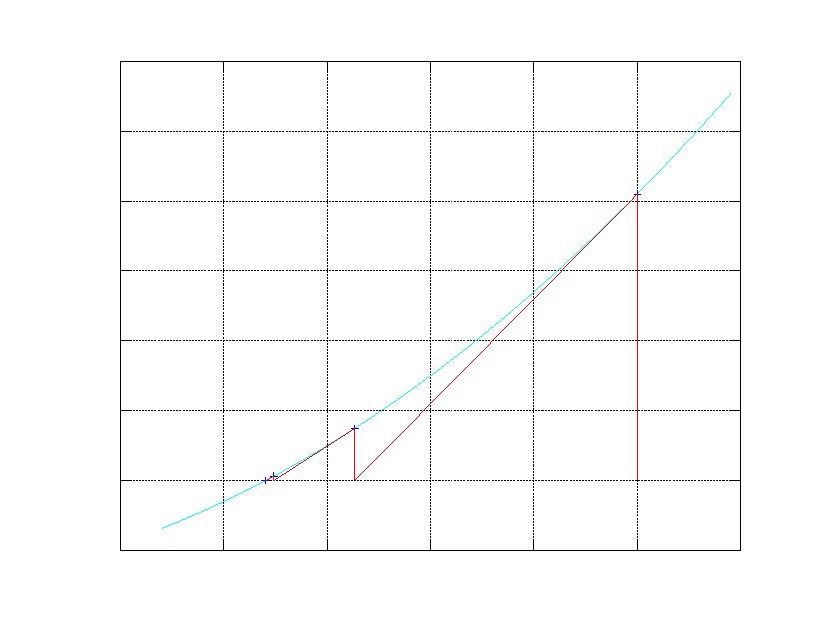
\includegraphics{RadiciEquazione/newton/newtonPlotOutput}}%
    \gplfronttext
  \end{picture}%
\endgroup

\end{center}

\begin{oss}
Per l'applicazione eseguita sopra ho utilizzato il criterio di arresto
\emph{incremento}, il metodo converge, ma posso studiare il condizionamento che
affetta ogni valutazione della precisione richiesta. Questo il codice che
dimostra questo condizionamento, comparando l'applicazione del metodo usando il
criterio di arresto per \emph{residuo}:
\begin{lstlisting}
[x, i, incAscisse, incChecked] = newtonMethod('singleZero','singleZeroDerivative', 7, 1e2, 10^(-14), 10^(-14), 'incrementCriterion');
octave:138> i
i =  5.00000000000000e+00
octave:139> errors = errorMonitor(incAscisse)
errors =
   4.12195121951219e+00   9.88875669244497e+00   8.93522817393261e+01   8.95110152113953e+03   9.18666331414061e+07   7.66765947567831e+15
octave:140> incChecked 
incChecked =
   2.73333333333333e+00   7.83682983682984e-01   7.70978577615202e-02   7.60913136916397e-04   7.41319183816813e-08   8.88178419700125e-16
octave:141> [x, i, resAscisse, resChecked] = newtonMethod('singleZero','singleZeroDerivative', 7, 1e2, 10^(-14), 10^(-14), 'residueCriterion');
octave:142> resChecked 
resChecked =
   2.73333333333333e+00   7.83682983682984e-01   7.70978577615201e-02   7.60913136916414e-04   7.41319183470686e-08   6.82317562092805e-16
octave:143> i
i =  5.00000000000000e+00
\end{lstlisting}
Si osserva che i valori utilizzati nel controllo per il raggiungimento della
precisione richiesta sono uguali tranne l'ultimo, il metodo che usa il criterio
\emph{residueCriterion} \`e pi\`u accurato, in quanto non \`e affetto dalla
cancellazione numerica (per l'ultima coppia di ascisse trovata il fattore di
amplificazione \`e $k = 7.66765947567831e+15$). 

I due metodi utilizzano comunque
lo stesso numero di passi per convergere alla soluzione.
\end{oss}

\begin{oss}
Posso effettuare una nuova comparazione: se chiedo una precisione di $tol_{X}
= 1e-16$, si osserva che il metodo non converge se si utilizza il criterio di 
arresto per \emph{incremento}, mentre converge usando il criterio per
\emph{residuo}. Questo il codice che dimostra quanto detto:
\begin{lstlisting}
octave:5> [x, i]=newtonMethod('singleZero','singleZeroDerivative', 7, 1e2, 10^(-16), 10^(-16),'incrementCriterion');
Il metodo non converge.
octave:6> [x, i]=newtonMethod('singleZero','singleZeroDerivative', 7, 1e2, 10^(-16), 10^(-16),'residueCriterion');
octave:7> i
i =  6
octave:8>
\end{lstlisting}
A parit\`a di numero massimo di passi, il secondo criterio permette al metodo di
convergere.
\end{oss}


\begin{exercise}
Implementare il metodo di newton ed applicarlo alla funzione \emph{functionWithNoRealZero},
con innesco iniziale $x_{0} = 2.5$, una tollerenza assoluta e relativa
$tol_{X} = rTol_{X} = 10^{-14}$ ed un numero massimo di iterazioni
$i_{max} = 7$.
\end{exercise}
Per l'implementazione del codice vedere \nameref{sec:newtonIterativeMethod}.
\begin{lstlisting}
octave:112> [x, i, ascisse] =
newtonMethod('functionWithNoRealZero','functionWithNoRealZeroDerivative', 2.5, 7, 1e-14, 1e-14, 'incrementCriterion') 
Il metodo non converge.
x = -3.18786023393994e+00
i =  7.00000000000000e+00
ascisse = [too long to report here]
octave:113> xNoZero = min(ascisse)-1:0.1:max(ascisse)+1
octave:114> yNoZero = invokeDelegate('functionWithNoRealZero', xNoZero)
octave:115> [prepX, prepY] = prepareForPlottingMethodSegments(ascisse, 'invokeDelegate', 'functionWithNoRealZero')
octave:116> plot(xNoZero, yNoZero, "c", ascisse,invokeDelegate('functionWithNoRealZero', ascisse), "b+", prepX, prepY, "r")
octave:117> grid
octave:118> print 'newtonNoZeroPlotOutput.tex' '-dTex' '-S800, 600'
\end{lstlisting}
Non si raggiunge la convergenza, infatti vengono fatti il massimo possibile
dei passi fissati dal parametro $i_{max}$. Questo l'output del comando \emph{octave:118}:
\begin{center}
% GNUPLOT: LaTeX picture with Postscript
\begingroup
  \makeatletter
  \providecommand\color[2][]{%
    \GenericError{(gnuplot) \space\space\space\@spaces}{%
      Package color not loaded in conjunction with
      terminal option `colourtext'%
    }{See the gnuplot documentation for explanation.%
    }{Either use 'blacktext' in gnuplot or load the package
      color.sty in LaTeX.}%
    \renewcommand\color[2][]{}%
  }%
  \providecommand\includegraphics[2][]{%
    \GenericError{(gnuplot) \space\space\space\@spaces}{%
      Package graphicx or graphics not loaded%
    }{See the gnuplot documentation for explanation.%
    }{The gnuplot epslatex terminal needs graphicx.sty or graphics.sty.}%
    \renewcommand\includegraphics[2][]{}%
  }%
  \providecommand\rotatebox[2]{#2}%
  \@ifundefined{ifGPcolor}{%
    \newif\ifGPcolor
    \GPcolortrue
  }{}%
  \@ifundefined{ifGPblacktext}{%
    \newif\ifGPblacktext
    \GPblacktexttrue
  }{}%
  % define a \g@addto@macro without @ in the name:
  \let\gplgaddtomacro\g@addto@macro
  % define empty templates for all commands taking text:
  \gdef\gplbacktext{}%
  \gdef\gplfronttext{}%
  \makeatother
  \ifGPblacktext
    % no textcolor at all
    \def\colorrgb#1{}%
    \def\colorgray#1{}%
  \else
    % gray or color?
    \ifGPcolor
      \def\colorrgb#1{\color[rgb]{#1}}%
      \def\colorgray#1{\color[gray]{#1}}%
      \expandafter\def\csname LTw\endcsname{\color{white}}%
      \expandafter\def\csname LTb\endcsname{\color{black}}%
      \expandafter\def\csname LTa\endcsname{\color{black}}%
      \expandafter\def\csname LT0\endcsname{\color[rgb]{1,0,0}}%
      \expandafter\def\csname LT1\endcsname{\color[rgb]{0,1,0}}%
      \expandafter\def\csname LT2\endcsname{\color[rgb]{0,0,1}}%
      \expandafter\def\csname LT3\endcsname{\color[rgb]{1,0,1}}%
      \expandafter\def\csname LT4\endcsname{\color[rgb]{0,1,1}}%
      \expandafter\def\csname LT5\endcsname{\color[rgb]{1,1,0}}%
      \expandafter\def\csname LT6\endcsname{\color[rgb]{0,0,0}}%
      \expandafter\def\csname LT7\endcsname{\color[rgb]{1,0.3,0}}%
      \expandafter\def\csname LT8\endcsname{\color[rgb]{0.5,0.5,0.5}}%
    \else
      % gray
      \def\colorrgb#1{\color{black}}%
      \def\colorgray#1{\color[gray]{#1}}%
      \expandafter\def\csname LTw\endcsname{\color{white}}%
      \expandafter\def\csname LTb\endcsname{\color{black}}%
      \expandafter\def\csname LTa\endcsname{\color{black}}%
      \expandafter\def\csname LT0\endcsname{\color{black}}%
      \expandafter\def\csname LT1\endcsname{\color{black}}%
      \expandafter\def\csname LT2\endcsname{\color{black}}%
      \expandafter\def\csname LT3\endcsname{\color{black}}%
      \expandafter\def\csname LT4\endcsname{\color{black}}%
      \expandafter\def\csname LT5\endcsname{\color{black}}%
      \expandafter\def\csname LT6\endcsname{\color{black}}%
      \expandafter\def\csname LT7\endcsname{\color{black}}%
      \expandafter\def\csname LT8\endcsname{\color{black}}%
    \fi
  \fi
  \setlength{\unitlength}{0.0500bp}%
  \begin{picture}(7680.00,5760.00)%
    \gplgaddtomacro\gplbacktext{%
      \colorrgb{0.00,0.00,0.00}%
      \put(866,634){\makebox(0,0)[r]{\strut{}0}}%
      \colorrgb{0.00,0.00,0.00}%
      \put(866,1807){\makebox(0,0)[r]{\strut{}5}}%
      \colorrgb{0.00,0.00,0.00}%
      \put(866,2981){\makebox(0,0)[r]{\strut{}10}}%
      \colorrgb{0.00,0.00,0.00}%
      \put(866,4154){\makebox(0,0)[r]{\strut{}15}}%
      \colorrgb{0.00,0.00,0.00}%
      \put(866,5327){\makebox(0,0)[r]{\strut{}20}}%
      \colorrgb{0.00,0.00,0.00}%
      \put(998,414){\makebox(0,0){\strut{}-6}}%
      \colorrgb{0.00,0.00,0.00}%
      \put(2188,414){\makebox(0,0){\strut{}-4}}%
      \colorrgb{0.00,0.00,0.00}%
      \put(3379,414){\makebox(0,0){\strut{}-2}}%
      \colorrgb{0.00,0.00,0.00}%
      \put(4569,414){\makebox(0,0){\strut{}0}}%
      \colorrgb{0.00,0.00,0.00}%
      \put(5760,414){\makebox(0,0){\strut{}2}}%
      \colorrgb{0.00,0.00,0.00}%
      \put(6950,414){\makebox(0,0){\strut{}4}}%
    }%
    \gplgaddtomacro\gplfronttext{%
    }%
    \gplbacktext
    \put(0,0){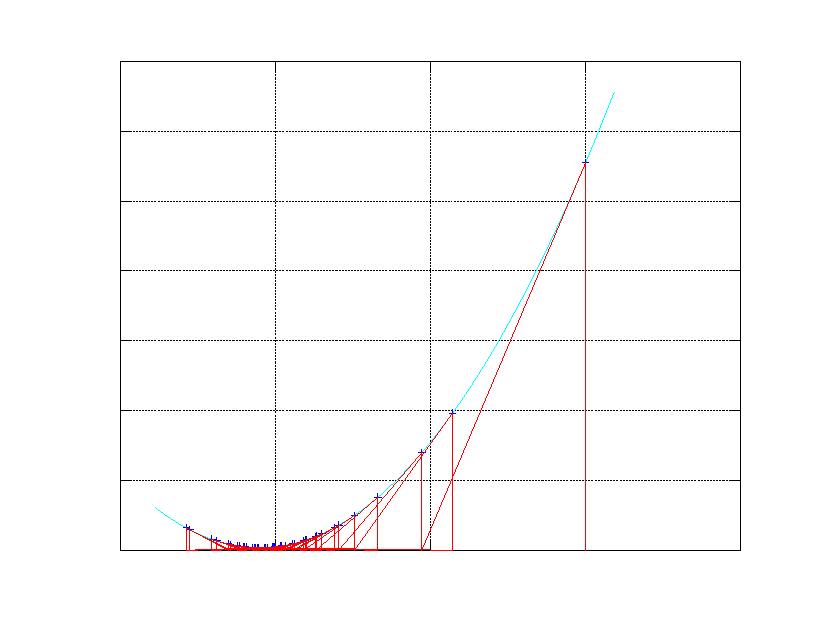
\includegraphics{RadiciEquazione/newton/newtonNoZeroPlotOutput}}%
    \gplfronttext
  \end{picture}%
\endgroup

\end{center}

\begin{exercise}[2.4]
\label{exercise:newtonLoopStartingPoint}
Per il testo dell'esercizio consultare il libro di testo.
\end{exercise}
Per l'implementazione del codice vedere \nameref{sec:newtonIterativeMethod}.

Nel primo caso studio il punto di innesco $x_{0} = 10$:
\begin{lstlisting}
octave:112> [x, i, ascisse] =
newtonMethod('functionNewtonRecursion','functionNewtonRecursionDerivative', 10, 5e1, 1e-14, 1e-14, 'incrementCriterion') 
x =  2.23606797749979e+00
i =  9.00000000000000e+00
ascisse = [too long to report here]
octave:113> xNoZero = min(ascisse)-1:0.1:max(ascisse)+1
octave:114> yNoZero = invokeDelegate('functionNewtonRecursion', xNoZero)
octave:115> [prepX, prepY] = prepareForPlottingMethodSegments(ascisse, 'invokeDelegate', 'functionNewtonRecursion')
octave:116> plot(xNoZero, yNoZero, "c", ascisse,invokeDelegate('functionNewtonRecursion', ascisse), "b+", prepX, prepY, "r")
octave:117> grid
octave:118> print 'newtonRecursivePlotOutput.tex' '-dTex' '-S800, 600'
\end{lstlisting}
Si raggiunge la convergenza con 9 passi. Questo l'output del comando
\emph{octave:118}:
\begin{center}
% GNUPLOT: LaTeX picture with Postscript
\begingroup
  \makeatletter
  \providecommand\color[2][]{%
    \GenericError{(gnuplot) \space\space\space\@spaces}{%
      Package color not loaded in conjunction with
      terminal option `colourtext'%
    }{See the gnuplot documentation for explanation.%
    }{Either use 'blacktext' in gnuplot or load the package
      color.sty in LaTeX.}%
    \renewcommand\color[2][]{}%
  }%
  \providecommand\includegraphics[2][]{%
    \GenericError{(gnuplot) \space\space\space\@spaces}{%
      Package graphicx or graphics not loaded%
    }{See the gnuplot documentation for explanation.%
    }{The gnuplot epslatex terminal needs graphicx.sty or graphics.sty.}%
    \renewcommand\includegraphics[2][]{}%
  }%
  \providecommand\rotatebox[2]{#2}%
  \@ifundefined{ifGPcolor}{%
    \newif\ifGPcolor
    \GPcolortrue
  }{}%
  \@ifundefined{ifGPblacktext}{%
    \newif\ifGPblacktext
    \GPblacktexttrue
  }{}%
  % define a \g@addto@macro without @ in the name:
  \let\gplgaddtomacro\g@addto@macro
  % define empty templates for all commands taking text:
  \gdef\gplbacktext{}%
  \gdef\gplfronttext{}%
  \makeatother
  \ifGPblacktext
    % no textcolor at all
    \def\colorrgb#1{}%
    \def\colorgray#1{}%
  \else
    % gray or color?
    \ifGPcolor
      \def\colorrgb#1{\color[rgb]{#1}}%
      \def\colorgray#1{\color[gray]{#1}}%
      \expandafter\def\csname LTw\endcsname{\color{white}}%
      \expandafter\def\csname LTb\endcsname{\color{black}}%
      \expandafter\def\csname LTa\endcsname{\color{black}}%
      \expandafter\def\csname LT0\endcsname{\color[rgb]{1,0,0}}%
      \expandafter\def\csname LT1\endcsname{\color[rgb]{0,1,0}}%
      \expandafter\def\csname LT2\endcsname{\color[rgb]{0,0,1}}%
      \expandafter\def\csname LT3\endcsname{\color[rgb]{1,0,1}}%
      \expandafter\def\csname LT4\endcsname{\color[rgb]{0,1,1}}%
      \expandafter\def\csname LT5\endcsname{\color[rgb]{1,1,0}}%
      \expandafter\def\csname LT6\endcsname{\color[rgb]{0,0,0}}%
      \expandafter\def\csname LT7\endcsname{\color[rgb]{1,0.3,0}}%
      \expandafter\def\csname LT8\endcsname{\color[rgb]{0.5,0.5,0.5}}%
    \else
      % gray
      \def\colorrgb#1{\color{black}}%
      \def\colorgray#1{\color[gray]{#1}}%
      \expandafter\def\csname LTw\endcsname{\color{white}}%
      \expandafter\def\csname LTb\endcsname{\color{black}}%
      \expandafter\def\csname LTa\endcsname{\color{black}}%
      \expandafter\def\csname LT0\endcsname{\color{black}}%
      \expandafter\def\csname LT1\endcsname{\color{black}}%
      \expandafter\def\csname LT2\endcsname{\color{black}}%
      \expandafter\def\csname LT3\endcsname{\color{black}}%
      \expandafter\def\csname LT4\endcsname{\color{black}}%
      \expandafter\def\csname LT5\endcsname{\color{black}}%
      \expandafter\def\csname LT6\endcsname{\color{black}}%
      \expandafter\def\csname LT7\endcsname{\color{black}}%
      \expandafter\def\csname LT8\endcsname{\color{black}}%
    \fi
  \fi
  \setlength{\unitlength}{0.0500bp}%
  \begin{picture}(7680.00,5760.00)%
    \gplgaddtomacro\gplbacktext{%
      \colorrgb{0.00,0.00,0.00}%
      \put(866,634){\makebox(0,0)[r]{\strut{}-500}}%
      \colorrgb{0.00,0.00,0.00}%
      \put(866,1807){\makebox(0,0)[r]{\strut{}0}}%
      \colorrgb{0.00,0.00,0.00}%
      \put(866,2981){\makebox(0,0)[r]{\strut{}500}}%
      \colorrgb{0.00,0.00,0.00}%
      \put(866,4154){\makebox(0,0)[r]{\strut{}1000}}%
      \colorrgb{0.00,0.00,0.00}%
      \put(866,5327){\makebox(0,0)[r]{\strut{}1500}}%
      \colorrgb{0.00,0.00,0.00}%
      \put(998,414){\makebox(0,0){\strut{}0}}%
      \colorrgb{0.00,0.00,0.00}%
      \put(1990,414){\makebox(0,0){\strut{}2}}%
      \colorrgb{0.00,0.00,0.00}%
      \put(2982,414){\makebox(0,0){\strut{}4}}%
      \colorrgb{0.00,0.00,0.00}%
      \put(3974,414){\makebox(0,0){\strut{}6}}%
      \colorrgb{0.00,0.00,0.00}%
      \put(4966,414){\makebox(0,0){\strut{}8}}%
      \colorrgb{0.00,0.00,0.00}%
      \put(5958,414){\makebox(0,0){\strut{}10}}%
      \colorrgb{0.00,0.00,0.00}%
      \put(6950,414){\makebox(0,0){\strut{}12}}%
    }%
    \gplgaddtomacro\gplfronttext{%
    }%
    \gplbacktext
    \put(0,0){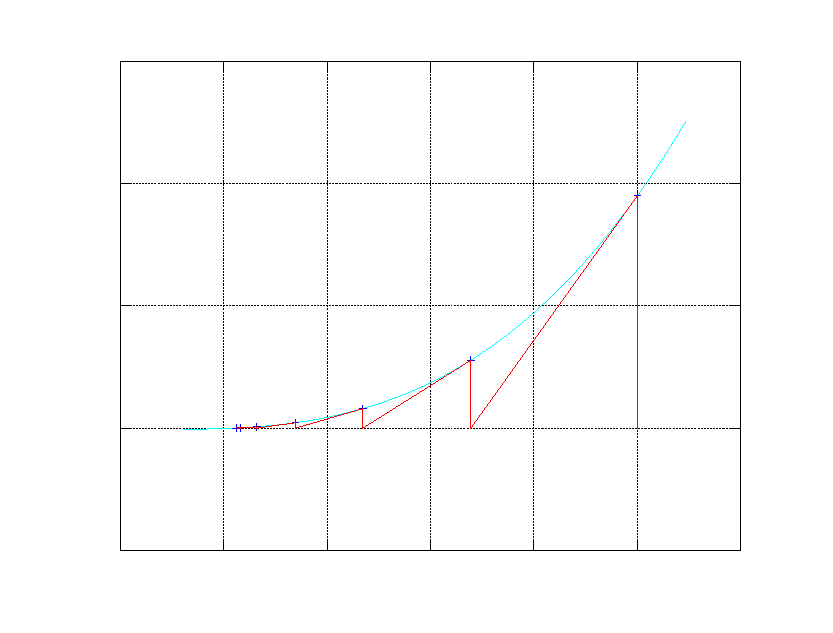
\includegraphics{RadiciEquazione/newton/newtonRecursivePlotOutput}}%
    \gplfronttext
  \end{picture}%
\endgroup

\end{center}

Nel secondo caso studio il punto di innesco $x_{0} = 1$:
\begin{lstlisting}
octave:112> [x, i, ascisse] =
newtonMethod('functionNewtonRecursion','functionNewtonRecursionDerivative', 1, 5e1, 1e-14, 1e-14, 'incrementCriterion') 
Il metodo non converge.
x = -1.00000000000000e+00
i =  5.00000000000000e+01
ascisse = [too long to report here]
octave:113> xNoZero = min(ascisse)-1:0.1:max(ascisse)+1
octave:114> yNoZero = invokeDelegate('functionNewtonRecursion', xNoZero)
octave:115> [prepX, prepY] = prepareForPlottingMethodSegments(ascisse, 'invokeDelegate', 'functionNewtonRecursion')
octave:116> plot(xNoZero, yNoZero, "c", ascisse,invokeDelegate('functionNewtonRecursion', ascisse), "b+", prepX, prepY, "r")
octave:117> grid
octave:118> print 'newtonRecursiveNotConvergencePlotOutput.tex' '-dTex' '-S800,600'
\end{lstlisting}
Il metodo non converge creando una finestra come si vede nel grafico. Questo
l'output del comando \emph{octave:118}:
\begin{center}
% GNUPLOT: LaTeX picture with Postscript
\begingroup
  \makeatletter
  \providecommand\color[2][]{%
    \GenericError{(gnuplot) \space\space\space\@spaces}{%
      Package color not loaded in conjunction with
      terminal option `colourtext'%
    }{See the gnuplot documentation for explanation.%
    }{Either use 'blacktext' in gnuplot or load the package
      color.sty in LaTeX.}%
    \renewcommand\color[2][]{}%
  }%
  \providecommand\includegraphics[2][]{%
    \GenericError{(gnuplot) \space\space\space\@spaces}{%
      Package graphicx or graphics not loaded%
    }{See the gnuplot documentation for explanation.%
    }{The gnuplot epslatex terminal needs graphicx.sty or graphics.sty.}%
    \renewcommand\includegraphics[2][]{}%
  }%
  \providecommand\rotatebox[2]{#2}%
  \@ifundefined{ifGPcolor}{%
    \newif\ifGPcolor
    \GPcolortrue
  }{}%
  \@ifundefined{ifGPblacktext}{%
    \newif\ifGPblacktext
    \GPblacktexttrue
  }{}%
  % define a \g@addto@macro without @ in the name:
  \let\gplgaddtomacro\g@addto@macro
  % define empty templates for all commands taking text:
  \gdef\gplbacktext{}%
  \gdef\gplfronttext{}%
  \makeatother
  \ifGPblacktext
    % no textcolor at all
    \def\colorrgb#1{}%
    \def\colorgray#1{}%
  \else
    % gray or color?
    \ifGPcolor
      \def\colorrgb#1{\color[rgb]{#1}}%
      \def\colorgray#1{\color[gray]{#1}}%
      \expandafter\def\csname LTw\endcsname{\color{white}}%
      \expandafter\def\csname LTb\endcsname{\color{black}}%
      \expandafter\def\csname LTa\endcsname{\color{black}}%
      \expandafter\def\csname LT0\endcsname{\color[rgb]{1,0,0}}%
      \expandafter\def\csname LT1\endcsname{\color[rgb]{0,1,0}}%
      \expandafter\def\csname LT2\endcsname{\color[rgb]{0,0,1}}%
      \expandafter\def\csname LT3\endcsname{\color[rgb]{1,0,1}}%
      \expandafter\def\csname LT4\endcsname{\color[rgb]{0,1,1}}%
      \expandafter\def\csname LT5\endcsname{\color[rgb]{1,1,0}}%
      \expandafter\def\csname LT6\endcsname{\color[rgb]{0,0,0}}%
      \expandafter\def\csname LT7\endcsname{\color[rgb]{1,0.3,0}}%
      \expandafter\def\csname LT8\endcsname{\color[rgb]{0.5,0.5,0.5}}%
    \else
      % gray
      \def\colorrgb#1{\color{black}}%
      \def\colorgray#1{\color[gray]{#1}}%
      \expandafter\def\csname LTw\endcsname{\color{white}}%
      \expandafter\def\csname LTb\endcsname{\color{black}}%
      \expandafter\def\csname LTa\endcsname{\color{black}}%
      \expandafter\def\csname LT0\endcsname{\color{black}}%
      \expandafter\def\csname LT1\endcsname{\color{black}}%
      \expandafter\def\csname LT2\endcsname{\color{black}}%
      \expandafter\def\csname LT3\endcsname{\color{black}}%
      \expandafter\def\csname LT4\endcsname{\color{black}}%
      \expandafter\def\csname LT5\endcsname{\color{black}}%
      \expandafter\def\csname LT6\endcsname{\color{black}}%
      \expandafter\def\csname LT7\endcsname{\color{black}}%
      \expandafter\def\csname LT8\endcsname{\color{black}}%
    \fi
  \fi
  \setlength{\unitlength}{0.0500bp}%
  \begin{picture}(7680.00,5760.00)%
    \gplgaddtomacro\gplbacktext{%
      \colorrgb{0.00,0.00,0.00}%
      \put(866,634){\makebox(0,0)[r]{\strut{}-6}}%
      \colorrgb{0.00,0.00,0.00}%
      \put(866,1416){\makebox(0,0)[r]{\strut{}-4}}%
      \colorrgb{0.00,0.00,0.00}%
      \put(866,2198){\makebox(0,0)[r]{\strut{}-2}}%
      \colorrgb{0.00,0.00,0.00}%
      \put(866,2981){\makebox(0,0)[r]{\strut{}0}}%
      \colorrgb{0.00,0.00,0.00}%
      \put(866,3763){\makebox(0,0)[r]{\strut{}2}}%
      \colorrgb{0.00,0.00,0.00}%
      \put(866,4545){\makebox(0,0)[r]{\strut{}4}}%
      \colorrgb{0.00,0.00,0.00}%
      \put(866,5327){\makebox(0,0)[r]{\strut{}6}}%
      \colorrgb{0.00,0.00,0.00}%
      \put(998,414){\makebox(0,0){\strut{}-2}}%
      \colorrgb{0.00,0.00,0.00}%
      \put(1742,414){\makebox(0,0){\strut{}-1.5}}%
      \colorrgb{0.00,0.00,0.00}%
      \put(2486,414){\makebox(0,0){\strut{}-1}}%
      \colorrgb{0.00,0.00,0.00}%
      \put(3230,414){\makebox(0,0){\strut{}-0.5}}%
      \colorrgb{0.00,0.00,0.00}%
      \put(3974,414){\makebox(0,0){\strut{}0}}%
      \colorrgb{0.00,0.00,0.00}%
      \put(4718,414){\makebox(0,0){\strut{}0.5}}%
      \colorrgb{0.00,0.00,0.00}%
      \put(5462,414){\makebox(0,0){\strut{}1}}%
      \colorrgb{0.00,0.00,0.00}%
      \put(6206,414){\makebox(0,0){\strut{}1.5}}%
      \colorrgb{0.00,0.00,0.00}%
      \put(6950,414){\makebox(0,0){\strut{}2}}%
    }%
    \gplgaddtomacro\gplfronttext{%
    }%
    \gplbacktext
    \put(0,0){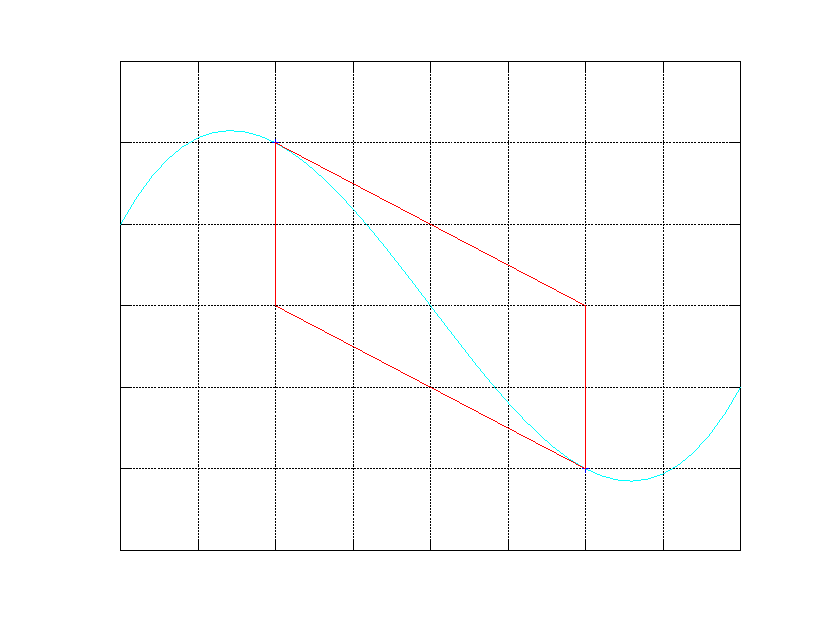
\includegraphics{RadiciEquazione/newton/newtonRecursiveNotConvergencePlotOutput}}%
    \gplfronttext
  \end{picture}%
\endgroup

\end{center}
\section{Varianti del metodo di Newton}
\label{sec:variantsMetodoDiNewton}

\begin{exercise}[2.5]
Per il testo dell'esercizio consultare il libro di testo.
\end{exercise}

Per l'implementazione del codice vedere \nameref{sec:newtonIterativeMethod},
\nameref{subsec:newtonMethodMultKnown},
\\\nameref{subsec:newtonMethodMultKnownLinearStopCriteria},
\nameref{subsec:newtonMethodAitken}.

I seguenti risultati sono stati generati invocando lo script
\nameref{subsec:ScriptEser25}:
\begin{lstlisting}
octave:221> scriptExercise25
\end{lstlisting}

Nella seguente tabella riporto l'applicazione dei metodi richiesti:
% i valori della seguente tabella sono stati presi dai dettagli inseriti nel
% file 'outputScriptExercise25.tex'
\begin{center}
\begin{tabular}{|c|c|c||c|c|}
\cline{2-5}
 \multicolumn{1}{c}{} &
 \multicolumn{2}{|c||}{function25first} &
 \multicolumn{2}{c|}{function25second}
 \\
\cline{2-5}
	\multicolumn{5}{c}{\textbf{Newton standard}} \\
\hline
	$tol_{X}$ & steps & x & steps & x \\
\hline
	$0.01$ & $3.60000000000000e+01$ & $1.18248003631401e+00$ &
	$4.50000000000000e+01$ & $1.18529447118482e+00$ \\
		
	$0.0001$ & $8.00000000000000e+01$ & $1.00176964345428e+00$ & 
	$9.00000000000000e+01$ & $1.00165056388247e+00$ \\

	$1e-06$ & $1.24000000000000e+02$ & $1.00001716153733e+00$ &
	$1.33000000000000e+02$ & $1.00001778848790e+00$ \\

	$1e-08$ & $1.68000000000000e+02$ & $1.00000016642808e+00$ & 
	$1.77000000000000e+02$ & $1.00000017250842e+00$ \\ 

	$1e-10$ & $2.11000000000000e+02$ & $1.00000000179331e+00$ & 
	$2.21000000000000e+02$ & $1.00000000167294e+00$ \\

	$1e-12$ & $2.55000000000000e+02$ & $1.00000000001739e+00$ & 
	$2.65000000000000e+02$ & $1.00000000001622e+00$ \\

	$1e-14$ & $2.99000000000000e+02$ & $1.00000000000017e+00$ &
	$3.08000000000000e+02$ & $1.00000000000017e+00$ \\

	$1e-16$ & $3.48000000000000e+02$ & $1.00000000000000e+00$ & 
	$3.56000000000000e+02$ & $1.00000000000000e+00$ \\ 
\hline
	\multicolumn{5}{c}{\textbf{Newton modificato}} \\
\hline
	$tol_{X}$ & steps & x & steps & x \\
\hline
	$0.01$ & $1.00000000000000e+00$ & $1.00000000000000e+00$ &
	$4.00000000000000e+00$ & $1.00000041794715e+00$ \\
		
	$0.0001$ & $1.00000000000000e+00$ & $1.00000000000000e+00$ & 
	$5.00000000000000e+00$ & $1.00000000000002e+00$ \\

	$1e-06$ & $1.00000000000000e+00$ & $1.00000000000000e+00$ &
	$5.00000000000000e+00$ & $1.00000000000002e+00$ \\

	$1e-08$ & $1.00000000000000e+00$ & $1.00000000000000e+00$ & 
	$6.00000000000000e+00$ & $1.00000000000000e+00$ \\ 

	$1e-10$ & $1.00000000000000e+00$ & $1.00000000000000e+00$ &
	$6.00000000000000e+00$ & $1.00000000000000e+00$ \\ 

	$1e-12$ & $1.00000000000000e+00$ & $1.00000000000000e+00$ & 
	$6.00000000000000e+00$ & $1.00000000000000e+00$ \\ 

	$1e-14$ & $1.00000000000000e+00$ & $1.00000000000000e+00$ &
	$6.00000000000000e+00$ & $1.00000000000000e+00$ \\ 

	$1e-16$ & $1.00000000000000e+00$ & $1.00000000000000e+00$ &
	$7.00000000000000e+00$ & $1.00000000000000e+00$ \\ 
\hline
	\multicolumn{5}{c}{\textbf{Newton Aitken}} \\
\hline
	$tol_{X}$ & steps & x & steps & x \\
\hline
	$0.01$ & $2.00000000000000e+00$ & $1.00000000000000e+00$ &
	$6.00000000000000e+00$ & $9.99999983328898e-01$ \\
		
	$0.0001$ & $2.00000000000000e+00$ & $1.00000000000000e+00$ &
	$7.00000000000000e+00$ & $1.00000000000000e+00$ \\

	$1e-06$ & $2.00000000000000e+00$ & $1.00000000000000e+00$ &
	$7.00000000000000e+00$ & $1.00000000000000e+00$ \\

	$1e-08$ & $2.00000000000000e+00$ & $1.00000000000000e+00$ &
	$7.00000000000000e+00$ & $1.00000000000000e+00$ \\

	$1e-10$ & $2.00000000000000e+00$ & $1.00000000000000e+00$ &
	$8.00000000000000e+00$ & $1.00000000000000e+00$ \\

	$1e-12$ & $2.00000000000000e+00$ & $1.00000000000000e+00$ &
	$8.00000000000000e+00$ & $1.00000000000000e+00$ \\

	$1e-14$ & $3.00000000000000e+00$ & $1.00000000000000e+00$ &
	$8.00000000000000e+00$ & $1.00000000000000e+00$ \\

	$1e-16$ & $3.00000000000000e+00$ & $1.00000000000000e+00$ &
	$8.00000000000000e+00$ & $1.00000000000000e+00$ \\
\hline
\end{tabular}
\end{center}


\begin{exercise}[2.9]
Per il testo dell'esercizio consultare il libro di testo.
\end{exercise}
Tutti i codici riguardanti i metodi richiesti sono implementati per aumentare
la ``robustezza'' delle iterazioni. \footnote{chiedere se effettivamente \`e
vero}
